\chapter{深度学习概念与现有视频目标跟踪算法理论}
\section{深度学习基础概念}
深度学习(Deep Lrarning)是以深度神经网络为模型结构的机器学习算法\supercite{deng2014deep}。机器学习(Mechine Learning)通常指一些依靠计算机确定模型的建模方法。目前大多数机器学习算法还无法完全自行实现学习,通常只能在人为规定的模型下,针对某个小问题对特定的数据建模。
\par
机器学习,模式识别等学科最终试图解决的问题通常是建立模型,解决问题。如目标跟踪即可描述为输入是视频,输出是轨迹的问题。神经网络由于其优秀的非线性拟合能力,成为如今机器学习最常用的模型之一。
\subsection{神经网络}

\subsubsection{CNN:卷积神经网络}
\subsubsection{RNN:循环神经网络}
\subsubsection{反向传播求梯度法}

\section{视频跟踪算法}
\subsection{运动模型}
运动模型是用于描述目标的运动的模型.本文中运动模型蕴含的信息包括目标的运动与目标的形态变化.
\par
\begin{figure}[htbp!]
    \centering
    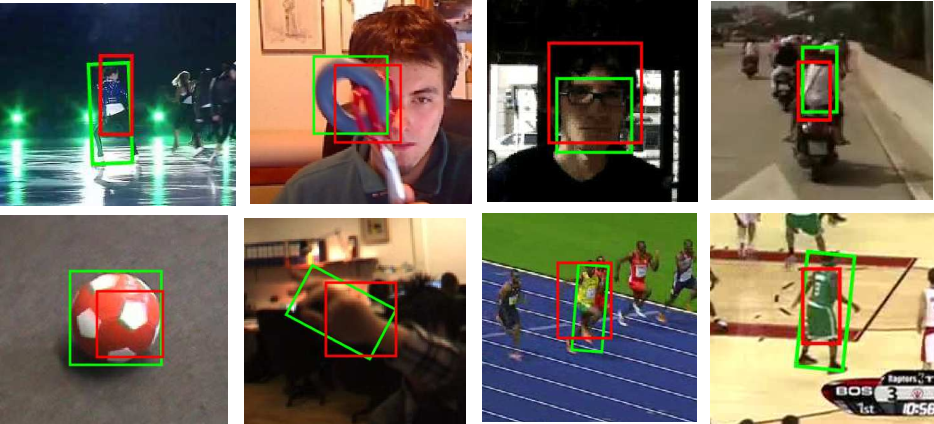
\includegraphics[width = 0.5\textwidth]{chap/img/overlap_examples.pdf}
    \caption{用于描述跟踪目标的外包矩形.红色:限定竖直的的外包矩形;绿色:不限定竖直的外包矩形.原图片为VOT竞赛中描述标记与目标的插图\supercite{VOT_TPAMI}}\label{fig:bunding_boxes}
\end{figure}
\par
常见的矩形框视频目标跟踪算法考虑会考虑目标的最小外包矩形(Bounding Box)和位置(Location).最小外包矩形的方向有时是限定为竖直的,即矩形的上下边平行于图像的上下边,左右边同理;有时不限定,可以是任何方向.限定竖直与不限定竖直的矩形表示法如图\ref{fig:bunding_boxes}所示.位置一般用矩形的中心表示.
\par
像素级跟踪算法的运动模型需要表达的信息与矩形框跟踪算法类似

\chapter{基于CNN和RNN的素级别跟踪算法}
本章是本文的重点,将详细介绍本研究的理论创新。
\par
本研究提出一种结合现有的像素级别处理技术和现有的矩形级视频目标跟踪技术的像素级别目标跟踪算法,具体算法结构,实现细节,训练等将在本章重点介绍.
\section{算法结构与核心思想}
本文所实现的算法将首先基于用于实现静态图像分割的U-Net\supercite{ronneberger2015u}的多级降级-升级卷机神经网络结构.但将在这个多级网络结构中加入Conv-LSTM结构.
\par
类似与U-Net的结构,本文的卷机网络部分也将有多个降级和升级结构;每个降级结构包括几个卷积层,使用池化结构进行降级;每个升级部分采用升卷积进行升级处理.在降级过程中,图片数据的尺寸大小会衰减,同时等比例增加其波段范围.对于3层的结构,最小级的波段将有128个.这个多级结构的设计理念是为了处理多尺度问题;浅层的级别能很好的处理细节问题,但对宏观的把控会较弱,具体表现为可能会出现噪声点;深层的结构对宏观把控好,但对边界处理较弱.升级结构能将浅层处理得到的边界信息与深层处理得到的宏观信息相结合,得到一个更好的结果.
\par
在时间尺度,本研究的算法将主要采用LSTM算法解决问题.具体的,LSTM单元将被加入到各个层级当中.LSTM在各种跟踪算法中有广泛应用,但大多数算法仅仅将其作为对最后结果的处理手段.本研究的算法将把LSTM作为所有的中间状态记录单元.
\par
与纽约大学2017年实现的Conv-LSTM结构的跟踪算法不同的是,本文所采用的多级神经网络将把Conv-LSTM加入各个卷机层级;而与U-Net,SegNet等多级分割算法不同的是,本文将在整个结构中多处穿插LSTM以得到一个时间连续的结果.
\section{基于CNN和RNN的像素级别跟踪模型在空间维度的处理}
\subsection{CNN的原理}
CNN是一种基于模板滤波的图像处理方法。常用的CNN的模板大小是$3*3$,有时也可以是$5*5$,$7*7$等大小
\subsection{多尺度思想的引入}
\section{基于CNN和RNN的像素级别跟踪模型在时间维度的处理}
\subsection{RNN的原理}
\subsection{跟踪状态}
\subsection{跟踪系统初始化}


% TODO 删除下边的,移到第三章
\section{模型训练}
本章前文中提出的模型结构是一个深度神经网络,它需要配合参数才可以运行.参数的获取过程称为模型训练.

\subsection{机器学习算法}

\subsection{模型训练原理}
模型训练(Train)是机器学习中获取参数的过程。典型的模型训练方法是梯度下降法。本研究的模型也将用梯度下降法求取参数。
\subsubsection{梯度下降法}

\subsubsection{求梯度:反向传播算法}
反向传播是常用的深度神经网络求梯度的方法。